\documentclass[1p]{elsarticle_modified}
%\bibliographystyle{elsarticle-num}

%\usepackage[colorlinks]{hyperref}
%\usepackage{abbrmath_seonhwa} %\Abb, \Ascr, \Acal ,\Abf, \Afrak
\usepackage{amsfonts}
\usepackage{amssymb}
\usepackage{amsmath}
\usepackage{amsthm}
\usepackage{scalefnt}
\usepackage{amsbsy}
\usepackage{kotex}
\usepackage{caption}
\usepackage{subfig}
\usepackage{color}
\usepackage{graphicx}
\usepackage{xcolor} %% white, black, red, green, blue, cyan, magenta, yellow
\usepackage{float}
\usepackage{setspace}
\usepackage{hyperref}

\usepackage{tikz}
\usetikzlibrary{arrows}

\usepackage{multirow}
\usepackage{array} % fixed length table
\usepackage{hhline}

%%%%%%%%%%%%%%%%%%%%%
\makeatletter
\renewcommand*\env@matrix[1][\arraystretch]{%
	\edef\arraystretch{#1}%
	\hskip -\arraycolsep
	\let\@ifnextchar\new@ifnextchar
	\array{*\c@MaxMatrixCols c}}
\makeatother %https://tex.stackexchange.com/questions/14071/how-can-i-increase-the-line-spacing-in-a-matrix
%%%%%%%%%%%%%%%

\usepackage[normalem]{ulem}

\newcommand{\msout}[1]{\ifmmode\text{\sout{\ensuremath{#1}}}\else\sout{#1}\fi}
%SOURCE: \msout is \stkout macro in https://tex.stackexchange.com/questions/20609/strikeout-in-math-mode

\newcommand{\cancel}[1]{
	\ifmmode
	{\color{red}\msout{#1}}
	\else
	{\color{red}\sout{#1}}
	\fi
}

\newcommand{\add}[1]{
	{\color{blue}\uwave{#1}}
}

\newcommand{\replace}[2]{
	\ifmmode
	{\color{red}\msout{#1}}{\color{blue}\uwave{#2}}
	\else
	{\color{red}\sout{#1}}{\color{blue}\uwave{#2}}
	\fi
}

\newcommand{\Sol}{\mathcal{S}} %segment
\newcommand{\D}{D} %diagram
\newcommand{\A}{\mathcal{A}} %arc


%%%%%%%%%%%%%%%%%%%%%%%%%%%%%5 test

\def\sl{\operatorname{\textup{SL}}(2,\Cbb)}
\def\psl{\operatorname{\textup{PSL}}(2,\Cbb)}
\def\quan{\mkern 1mu \triangleright \mkern 1mu}

\theoremstyle{definition}
\newtheorem{thm}{Theorem}[section]
\newtheorem{prop}[thm]{Proposition}
\newtheorem{lem}[thm]{Lemma}
\newtheorem{ques}[thm]{Question}
\newtheorem{cor}[thm]{Corollary}
\newtheorem{defn}[thm]{Definition}
\newtheorem{exam}[thm]{Example}
\newtheorem{rmk}[thm]{Remark}
\newtheorem{alg}[thm]{Algorithm}

\newcommand{\I}{\sqrt{-1}}
\begin{document}

%\begin{frontmatter}
%
%\title{Boundary parabolic representations of knots up to 8 crossings}
%
%%% Group authors per affiliation:
%\author{Yunhi Cho} 
%\address{Department of Mathematics, University of Seoul, Seoul, Korea}
%\ead{yhcho@uos.ac.kr}
%
%
%\author{Seonhwa Kim} %\fnref{s_kim}}
%\address{Center for Geometry and Physics, Institute for Basic Science, Pohang, 37673, Korea}
%\ead{ryeona17@ibs.re.kr}
%
%\author{Hyuk Kim}
%\address{Department of Mathematical Sciences, Seoul National University, Seoul 08826, Korea}
%\ead{hyukkim@snu.ac.kr}
%
%\author{Seokbeom Yoon}
%\address{Department of Mathematical Sciences, Seoul National University, Seoul, 08826,  Korea}
%\ead{sbyoon15@snu.ac.kr}
%
%\begin{abstract}
%We find all boundary parabolic representation of knots up to 8 crossings.
%
%\end{abstract}
%\begin{keyword}
%    \MSC[2010] 57M25 
%\end{keyword}
%
%\end{frontmatter}

%\linenumbers
%\tableofcontents
%
\newcommand\colored[1]{\textcolor{white}{\rule[-0.35ex]{0.8em}{1.4ex}}\kern-0.8em\color{red} #1}%
%\newcommand\colored[1]{\textcolor{white}{ #1}\kern-2.17ex	\textcolor{white}{ #1}\kern-1.81ex	\textcolor{white}{ #1}\kern-2.15ex\color{red}#1	}

{\Large $\underline{12a_{0702}~(K12a_{0702})}$}

\setlength{\tabcolsep}{10pt}
\renewcommand{\arraystretch}{1.6}
\vspace{1cm}\begin{tabular}{m{100pt}>{\centering\arraybackslash}m{274pt}}
\multirow{5}{120pt}{
	\centering
	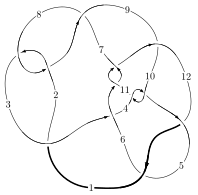
\includegraphics[width=112pt]{../../../GIT/diagram.site/Diagrams/png/1503_12a_0702.png}\\
\ \ \ A knot diagram\footnotemark}&
\allowdisplaybreaks
\textbf{Linearized knot diagam} \\
\cline{2-2}
 &
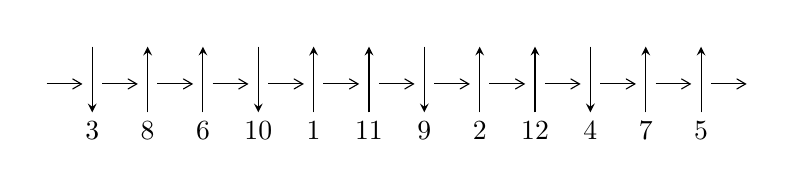
\begin{tikzpicture}[x=20pt, y=17pt]
	% nodes
	\node (C0) at (0, 0) {};
	\node (C1) at (1, 0) {};
	\node (C1U) at (1, +1) {};
	\node (C1D) at (1, -1) {3};

	\node (C2) at (2, 0) {};
	\node (C2U) at (2, +1) {};
	\node (C2D) at (2, -1) {8};

	\node (C3) at (3, 0) {};
	\node (C3U) at (3, +1) {};
	\node (C3D) at (3, -1) {6};

	\node (C4) at (4, 0) {};
	\node (C4U) at (4, +1) {};
	\node (C4D) at (4, -1) {10};

	\node (C5) at (5, 0) {};
	\node (C5U) at (5, +1) {};
	\node (C5D) at (5, -1) {1};

	\node (C6) at (6, 0) {};
	\node (C6U) at (6, +1) {};
	\node (C6D) at (6, -1) {11};

	\node (C7) at (7, 0) {};
	\node (C7U) at (7, +1) {};
	\node (C7D) at (7, -1) {9};

	\node (C8) at (8, 0) {};
	\node (C8U) at (8, +1) {};
	\node (C8D) at (8, -1) {2};

	\node (C9) at (9, 0) {};
	\node (C9U) at (9, +1) {};
	\node (C9D) at (9, -1) {12};

	\node (C10) at (10, 0) {};
	\node (C10U) at (10, +1) {};
	\node (C10D) at (10, -1) {4};

	\node (C11) at (11, 0) {};
	\node (C11U) at (11, +1) {};
	\node (C11D) at (11, -1) {7};

	\node (C12) at (12, 0) {};
	\node (C12U) at (12, +1) {};
	\node (C12D) at (12, -1) {5};
	\node (C13) at (13, 0) {};

	% arrows
	\draw[->,>={angle 60}]
	(C0) edge (C1) (C1) edge (C2) (C2) edge (C3) (C3) edge (C4) (C4) edge (C5) (C5) edge (C6) (C6) edge (C7) (C7) edge (C8) (C8) edge (C9) (C9) edge (C10) (C10) edge (C11) (C11) edge (C12) (C12) edge (C13) ;	\draw[->,>=stealth]
	(C1U) edge (C1D) (C2D) edge (C2U) (C3D) edge (C3U) (C4U) edge (C4D) (C5D) edge (C5U) (C6D) edge (C6U) (C7U) edge (C7D) (C8D) edge (C8U) (C9D) edge (C9U) (C10U) edge (C10D) (C11D) edge (C11U) (C12D) edge (C12U) ;
	\end{tikzpicture} \\
\hhline{~~} \\& 
\textbf{Solving Sequence} \\ \cline{2-2} 
 &
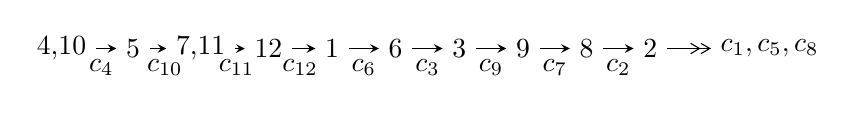
\begin{tikzpicture}[x=23pt, y=7pt]
	% node
	\node (A0) at (-1/8, 0) {4,10};
	\node (A1) at (1, 0) {5};
	\node (A2) at (33/16, 0) {7,11};
	\node (A3) at (25/8, 0) {12};
	\node (A4) at (33/8, 0) {1};
	\node (A5) at (41/8, 0) {6};
	\node (A6) at (49/8, 0) {3};
	\node (A7) at (57/8, 0) {9};
	\node (A8) at (65/8, 0) {8};
	\node (A9) at (73/8, 0) {2};
	\node (C1) at (1/2, -1) {$c_{4}$};
	\node (C2) at (3/2, -1) {$c_{10}$};
	\node (C3) at (21/8, -1) {$c_{11}$};
	\node (C4) at (29/8, -1) {$c_{12}$};
	\node (C5) at (37/8, -1) {$c_{6}$};
	\node (C6) at (45/8, -1) {$c_{3}$};
	\node (C7) at (53/8, -1) {$c_{9}$};
	\node (C8) at (61/8, -1) {$c_{7}$};
	\node (C9) at (69/8, -1) {$c_{2}$};
	\node (A10) at (11, 0) {$c_{1},c_{5},c_{8}$};

	% edge
	\draw[->,>=stealth]	
	(A0) edge (A1) (A1) edge (A2) (A2) edge (A3) (A3) edge (A4) (A4) edge (A5) (A5) edge (A6) (A6) edge (A7) (A7) edge (A8) (A8) edge (A9) ;
	\draw[->>,>={angle 60}]	
	(A9) edge (A10);
\end{tikzpicture} \\ 

\end{tabular} \\

\footnotetext{
The image of knot diagram is generated by the software ``\textbf{Draw programme}" developed by Andrew Bartholomew(\url{http://www.layer8.co.uk/maths/draw/index.htm\#Running-draw}), where we modified some parts for our purpose(\url{https://github.com/CATsTAILs/LinksPainter}).
}\phantom \\ \newline 
\centering \textbf{Ideals for irreducible components\footnotemark of $X_{\text{par}}$} 
 
\begin{align*}
I^u_{1}&=\langle 
-1.19038\times10^{83} u^{40}+4.26853\times10^{83} u^{39}+\cdots+1.55480\times10^{86} b-1.07861\times10^{86},\\
\phantom{I^u_{1}}&\phantom{= \langle  }-5.72981\times10^{85} u^{40}+1.60933\times10^{86} u^{39}+\cdots+3.88699\times10^{87} a-9.00245\times10^{87},\\
\phantom{I^u_{1}}&\phantom{= \langle  }u^{41}-3 u^{40}+\cdots-434 u+50\rangle \\
I^u_{2}&=\langle 
- u^2 a+b+1,\;-2 u^{26} a-2 u^{25} a+\cdots-3 a+6,\;u^{27}+u^{26}+\cdots+2 u-1\rangle \\
I^u_{3}&=\langle 
u^3- u^2+5 b+2 u+3,\;3 u^3+2 u^2+10 a-14 u-6,\;u^4-2 u^2+2\rangle \\
I^u_{4}&=\langle 
b+a-1,\;8 a^3+4 a^2 u-12 a^2-4 a u+2 a+1,\;u^2+1\rangle \\
\\
I^v_{1}&=\langle 
a,\;b+1,\;v+1\rangle \\
\end{align*}
\raggedright * 5 irreducible components of $\dim_{\mathbb{C}}=0$, with total 106 representations.\\
\footnotetext{All coefficients of polynomials are rational numbers. But the coefficients are sometimes approximated in decimal forms when there is not enough margin.}
\newpage
\renewcommand{\arraystretch}{1}
\centering \section*{I. $I^u_{1}= \langle -1.19\times10^{83} u^{40}+4.27\times10^{83} u^{39}+\cdots+1.55\times10^{86} b-1.08\times10^{86},\;-5.73\times10^{85} u^{40}+1.61\times10^{86} u^{39}+\cdots+3.89\times10^{87} a-9.00\times10^{87},\;u^{41}-3 u^{40}+\cdots-434 u+50 \rangle$}
\flushleft \textbf{(i) Arc colorings}\\
\begin{tabular}{m{7pt} m{180pt} m{7pt} m{180pt} }
\flushright $a_{4}=$&$\begin{pmatrix}1\\0\end{pmatrix}$ \\
\flushright $a_{10}=$&$\begin{pmatrix}0\\u\end{pmatrix}$ \\
\flushright $a_{5}=$&$\begin{pmatrix}1\\u^2\end{pmatrix}$ \\
\flushright $a_{7}=$&$\begin{pmatrix}0.0147410 u^{40}-0.0414030 u^{39}+\cdots+31.9284 u+2.31605\\0.000765620 u^{40}-0.00274539 u^{39}+\cdots+1.07683 u+0.693733\end{pmatrix}$ \\
\flushright $a_{11}=$&$\begin{pmatrix}- u\\u\end{pmatrix}$ \\
\flushright $a_{12}=$&$\begin{pmatrix}0.0115033 u^{40}-0.0353806 u^{39}+\cdots+46.5023 u-6.32310\\0.00230652 u^{40}-0.00672063 u^{39}+\cdots+8.78658 u-0.731794\end{pmatrix}$ \\
\flushright $a_{1}=$&$\begin{pmatrix}0.0138747 u^{40}-0.0423896 u^{39}+\cdots+56.2419 u-7.09843\\0.00281990 u^{40}-0.00776945 u^{39}+\cdots+8.71363 u-0.737049\end{pmatrix}$ \\
\flushright $a_{6}=$&$\begin{pmatrix}0.0146359 u^{40}-0.0416011 u^{39}+\cdots+31.6745 u+2.43461\\0.000870716 u^{40}-0.00254730 u^{39}+\cdots+1.33067 u+0.575165\end{pmatrix}$ \\
\flushright $a_{3}=$&$\begin{pmatrix}0.0128297 u^{40}-0.0366995 u^{39}+\cdots+28.5656 u+1.49810\\0.00113437 u^{40}-0.00267356 u^{39}+\cdots+2.04755 u+0.246021\end{pmatrix}$ \\
\flushright $a_{9}=$&$\begin{pmatrix}0.00492043 u^{40}-0.0158956 u^{39}+\cdots+24.8003 u-4.18302\\0.00178970 u^{40}-0.00537829 u^{39}+\cdots+7.06620 u-0.641486\end{pmatrix}$ \\
\flushright $a_{8}=$&$\begin{pmatrix}-0.000300319 u^{40}+0.00224674 u^{39}+\cdots-9.20295 u+3.52338\\-0.00108526 u^{40}+0.00257937 u^{39}+\cdots-2.40758 u+0.183564\end{pmatrix}$ \\
\flushright $a_{2}=$&$\begin{pmatrix}0.00367128 u^{40}-0.00992859 u^{39}+\cdots+5.43318 u+0.814239\\0.00134579 u^{40}-0.00361819 u^{39}+\cdots+3.39304 u+0.0150160\end{pmatrix}$\\&\end{tabular}
\flushleft \textbf{(ii) Obstruction class $= -1$}\\~\\
\flushleft \textbf{(iii) Cusp Shapes $= -0.0228051 u^{40}+0.0718802 u^{39}+\cdots-38.8520 u+4.20733$}\\~\\
\newpage\renewcommand{\arraystretch}{1}
\flushleft \textbf{(iv) u-Polynomials at the component}\newline \\
\begin{tabular}{m{50pt}|m{274pt}}
Crossings & \hspace{64pt}u-Polynomials at each crossing \\
\hline $$\begin{aligned}c_{1},c_{7}\end{aligned}$$&$\begin{aligned}
&u^{41}+13 u^{40}+\cdots-1260 u-100
\end{aligned}$\\
\hline $$\begin{aligned}c_{2},c_{8}\end{aligned}$$&$\begin{aligned}
&u^{41}+3 u^{40}+\cdots-10 u+10
\end{aligned}$\\
\hline $$\begin{aligned}c_{3},c_{9}\end{aligned}$$&$\begin{aligned}
&64(64 u^{41}+256 u^{40}+\cdots-13 u^2-1)
\end{aligned}$\\
\hline $$\begin{aligned}c_{4},c_{10}\end{aligned}$$&$\begin{aligned}
&u^{41}-3 u^{40}+\cdots-434 u+50
\end{aligned}$\\
\hline $$\begin{aligned}c_{5},c_{6},c_{11}\\c_{12}\end{aligned}$$&$\begin{aligned}
&u^{41}- u^{40}+\cdots+14 u-1
\end{aligned}$\\
\hline
\end{tabular}\\~\\
\newpage\renewcommand{\arraystretch}{1}
\flushleft \textbf{(v) Riley Polynomials at the component}\newline \\
\begin{tabular}{m{50pt}|m{274pt}}
Crossings & \hspace{64pt}Riley Polynomials at each crossing \\
\hline $$\begin{aligned}c_{1},c_{7}\end{aligned}$$&$\begin{aligned}
&y^{41}+33 y^{40}+\cdots-489200 y-10000
\end{aligned}$\\
\hline $$\begin{aligned}c_{2},c_{8}\end{aligned}$$&$\begin{aligned}
&y^{41}+13 y^{40}+\cdots-1260 y-100
\end{aligned}$\\
\hline $$\begin{aligned}c_{3},c_{9}\end{aligned}$$&$\begin{aligned}
&4096(4096 y^{41}-147456 y^{40}+\cdots-26 y-1)
\end{aligned}$\\
\hline $$\begin{aligned}c_{4},c_{10}\end{aligned}$$&$\begin{aligned}
&y^{41}+25 y^{40}+\cdots-199044 y-2500
\end{aligned}$\\
\hline $$\begin{aligned}c_{5},c_{6},c_{11}\\c_{12}\end{aligned}$$&$\begin{aligned}
&y^{41}-31 y^{40}+\cdots-96 y-1
\end{aligned}$\\
\hline
\end{tabular}\\~\\
\newpage\flushleft \textbf{(vi) Complex Volumes and Cusp Shapes}
$$\begin{array}{c|c|c}  
\text{Solutions to }I^u_{1}& \I (\text{vol} + \sqrt{-1}CS) & \text{Cusp shape}\\
 \hline 
\begin{aligned}
u &= \phantom{-}0.455951 + 0.852881 I \\
a &= \phantom{-}0.728739 + 0.291805 I \\
b &= \phantom{-}0.139910 - 0.558255 I\end{aligned}
 & \phantom{-}0.86494 + 1.62805 I & \phantom{-}5.67415 - 3.58289 I \\ \hline\begin{aligned}
u &= \phantom{-}0.455951 - 0.852881 I \\
a &= \phantom{-}0.728739 - 0.291805 I \\
b &= \phantom{-}0.139910 + 0.558255 I\end{aligned}
 & \phantom{-}0.86494 - 1.62805 I & \phantom{-}5.67415 + 3.58289 I \\ \hline\begin{aligned}
u &= -0.021368 + 1.036750 I \\
a &= \phantom{-}1.161860 + 0.121316 I \\
b &= -1.236090 - 0.167032 I\end{aligned}
 & \phantom{-}4.65548 + 2.80230 I & \phantom{-}13.48887 - 2.99820 I \\ \hline\begin{aligned}
u &= -0.021368 - 1.036750 I \\
a &= \phantom{-}1.161860 - 0.121316 I \\
b &= -1.236090 + 0.167032 I\end{aligned}
 & \phantom{-}4.65548 - 2.80230 I & \phantom{-}13.48887 + 2.99820 I \\ \hline\begin{aligned}
u &= -0.850702 + 0.604796 I \\
a &= \phantom{-}1.089290 - 0.351516 I \\
b &= -0.364276 + 0.545866 I\end{aligned}
 & -0.16962 + 2.89326 I & \phantom{-}2.19290 - 0.10248 I \\ \hline\begin{aligned}
u &= -0.850702 - 0.604796 I \\
a &= \phantom{-}1.089290 + 0.351516 I \\
b &= -0.364276 - 0.545866 I\end{aligned}
 & -0.16962 - 2.89326 I & \phantom{-}2.19290 + 0.10248 I \\ \hline\begin{aligned}
u &= -0.471844 + 0.764313 I \\
a &= -0.121231 + 0.155243 I \\
b &= \phantom{-}0.127637 - 0.862325 I\end{aligned}
 & \phantom{-}1.00547 + 1.41725 I & \phantom{-}6.32483 - 4.75240 I \\ \hline\begin{aligned}
u &= -0.471844 - 0.764313 I \\
a &= -0.121231 - 0.155243 I \\
b &= \phantom{-}0.127637 + 0.862325 I\end{aligned}
 & \phantom{-}1.00547 - 1.41725 I & \phantom{-}6.32483 + 4.75240 I \\ \hline\begin{aligned}
u &= \phantom{-}0.676505 + 0.580935 I \\
a &= -0.636641 + 0.057470 I \\
b &= \phantom{-}0.388189 + 0.860067 I\end{aligned}
 & -0.01909 - 5.83785 I & \phantom{-}3.11476 + 10.68510 I \\ \hline\begin{aligned}
u &= \phantom{-}0.676505 - 0.580935 I \\
a &= -0.636641 - 0.057470 I \\
b &= \phantom{-}0.388189 - 0.860067 I\end{aligned}
 & -0.01909 + 5.83785 I & \phantom{-}3.11476 - 10.68510 I\\
 \hline 
 \end{array}$$\newpage$$\begin{array}{c|c|c}  
\text{Solutions to }I^u_{1}& \I (\text{vol} + \sqrt{-1}CS) & \text{Cusp shape}\\
 \hline 
\begin{aligned}
u &= \phantom{-}0.106757 + 1.119200 I \\
a &= \phantom{-}0.407888 + 0.094333 I \\
b &= \phantom{-}0.707134 - 0.209548 I\end{aligned}
 & -0.743392 - 0.853731 I & \phantom{-}8.26894 + 8.56558 I \\ \hline\begin{aligned}
u &= \phantom{-}0.106757 - 1.119200 I \\
a &= \phantom{-}0.407888 - 0.094333 I \\
b &= \phantom{-}0.707134 + 0.209548 I\end{aligned}
 & -0.743392 + 0.853731 I & \phantom{-}8.26894 - 8.56558 I \\ \hline\begin{aligned}
u &= -0.135573 + 0.750401 I \\
a &= \phantom{-}0.497918 + 0.003694 I \\
b &= -0.087550 - 0.403450 I\end{aligned}
 & \phantom{-}0.517216 + 0.980568 I & \phantom{-}7.41204 - 7.03124 I \\ \hline\begin{aligned}
u &= -0.135573 - 0.750401 I \\
a &= \phantom{-}0.497918 - 0.003694 I \\
b &= -0.087550 + 0.403450 I\end{aligned}
 & \phantom{-}0.517216 - 0.980568 I & \phantom{-}7.41204 + 7.03124 I \\ \hline\begin{aligned}
u &= \phantom{-}0.015207 + 1.271930 I \\
a &= \phantom{-}0.258817 + 0.015105 I \\
b &= \phantom{-}1.052190 - 0.036306 I\end{aligned}
 & \phantom{-}4.96111 - 3.02863 I & \phantom{-}13.36303 + 2.94764 I \\ \hline\begin{aligned}
u &= \phantom{-}0.015207 - 1.271930 I \\
a &= \phantom{-}0.258817 - 0.015105 I \\
b &= \phantom{-}1.052190 + 0.036306 I\end{aligned}
 & \phantom{-}4.96111 + 3.02863 I & \phantom{-}13.36303 - 2.94764 I \\ \hline\begin{aligned}
u &= \phantom{-}1.267430 + 0.165148 I \\
a &= -1.57147 - 0.04495 I \\
b &= \phantom{-}0.523699 + 0.462735 I\end{aligned}
 & \phantom{-}10.5970 - 11.3672 I & \phantom{-}9.96311 + 7.10557 I \\ \hline\begin{aligned}
u &= \phantom{-}1.267430 - 0.165148 I \\
a &= -1.57147 + 0.04495 I \\
b &= \phantom{-}0.523699 - 0.462735 I\end{aligned}
 & \phantom{-}10.5970 + 11.3672 I & \phantom{-}9.96311 - 7.10557 I \\ \hline\begin{aligned}
u &= -1.303430 + 0.145939 I \\
a &= -1.59455 + 0.04931 I \\
b &= \phantom{-}0.546188 - 0.390643 I\end{aligned}
 & \phantom{-}11.47150 + 4.79100 I & \phantom{-}11.44614 - 2.44954 I \\ \hline\begin{aligned}
u &= -1.303430 - 0.145939 I \\
a &= -1.59455 - 0.04931 I \\
b &= \phantom{-}0.546188 + 0.390643 I\end{aligned}
 & \phantom{-}11.47150 - 4.79100 I & \phantom{-}11.44614 + 2.44954 I\\
 \hline 
 \end{array}$$\newpage$$\begin{array}{c|c|c}  
\text{Solutions to }I^u_{1}& \I (\text{vol} + \sqrt{-1}CS) & \text{Cusp shape}\\
 \hline 
\begin{aligned}
u &= -1.48598\phantom{ +0.000000I} \\
a &= -1.70628\phantom{ +0.000000I} \\
b &= \phantom{-}0.809440\phantom{ +0.000000I}\end{aligned}
 & \phantom{-}6.30192\phantom{ +0.000000I} & \phantom{-}14.4050\phantom{ +0.000000I} \\ \hline\begin{aligned}
u &= \phantom{-}0.346910 + 0.359461 I \\
a &= -0.044452 + 0.984431 I \\
b &= \phantom{-}0.444124 + 0.546475 I\end{aligned}
 & -2.78156 - 0.97104 I & -4.60139 + 3.38415 I \\ \hline\begin{aligned}
u &= \phantom{-}0.346910 - 0.359461 I \\
a &= -0.044452 - 0.984431 I \\
b &= \phantom{-}0.444124 - 0.546475 I\end{aligned}
 & -2.78156 + 0.97104 I & -4.60139 - 3.38415 I \\ \hline\begin{aligned}
u &= \phantom{-}1.54269 + 0.18278 I \\
a &= -1.72780 - 0.12223 I \\
b &= \phantom{-}0.941440 + 0.289062 I\end{aligned}
 & \phantom{-}2.02994 - 4.70447 I & \phantom{-}11.23439 + 5.82932 I \\ \hline\begin{aligned}
u &= \phantom{-}1.54269 - 0.18278 I \\
a &= -1.72780 + 0.12223 I \\
b &= \phantom{-}0.941440 - 0.289062 I\end{aligned}
 & \phantom{-}2.02994 + 4.70447 I & \phantom{-}11.23439 - 5.82932 I \\ \hline\begin{aligned}
u &= \phantom{-}0.52762 + 1.47752 I \\
a &= -0.21972 + 1.74763 I \\
b &= \phantom{-}0.20870 - 2.77021 I\end{aligned}
 & \phantom{-}15.8147 - 17.6250 I & \phantom{-0.000000 } 0 \\ \hline\begin{aligned}
u &= \phantom{-}0.52762 - 1.47752 I \\
a &= -0.21972 - 1.74763 I \\
b &= \phantom{-}0.20870 + 2.77021 I\end{aligned}
 & \phantom{-}15.8147 + 17.6250 I & \phantom{-0.000000 } 0 \\ \hline\begin{aligned}
u &= -0.53754 + 1.48742 I \\
a &= -0.19175 - 1.71682 I \\
b &= \phantom{-}0.21292 + 2.73453 I\end{aligned}
 & \phantom{-}16.6893 + 11.2011 I & \phantom{-0.000000 } 0 \\ \hline\begin{aligned}
u &= -0.53754 - 1.48742 I \\
a &= -0.19175 + 1.71682 I \\
b &= \phantom{-}0.21292 - 2.73453 I\end{aligned}
 & \phantom{-}16.6893 - 11.2011 I & \phantom{-0.000000 } 0 \\ \hline\begin{aligned}
u &= \phantom{-}0.50522 + 1.54544 I \\
a &= -0.04761 + 1.80771 I \\
b &= \phantom{-}0.06833 - 2.69458 I\end{aligned}
 & \phantom{-}7.92273 - 11.59880 I & \phantom{-0.000000 } 0\\
 \hline 
 \end{array}$$\newpage$$\begin{array}{c|c|c}  
\text{Solutions to }I^u_{1}& \I (\text{vol} + \sqrt{-1}CS) & \text{Cusp shape}\\
 \hline 
\begin{aligned}
u &= \phantom{-}0.50522 - 1.54544 I \\
a &= -0.04761 - 1.80771 I \\
b &= \phantom{-}0.06833 + 2.69458 I\end{aligned}
 & \phantom{-}7.92273 + 11.59880 I & \phantom{-0.000000 } 0 \\ \hline\begin{aligned}
u &= -0.56045 + 1.56650 I \\
a &= \phantom{-}0.03187 - 1.69887 I \\
b &= \phantom{-}0.08948 + 2.57599 I\end{aligned}
 & \phantom{-}11.62590 + 7.27779 I & \phantom{-0.000000 } 0 \\ \hline\begin{aligned}
u &= -0.56045 - 1.56650 I \\
a &= \phantom{-}0.03187 + 1.69887 I \\
b &= \phantom{-}0.08948 - 2.57599 I\end{aligned}
 & \phantom{-}11.62590 - 7.27779 I & \phantom{-0.000000 } 0 \\ \hline\begin{aligned}
u &= -0.68168 + 1.55704 I \\
a &= \phantom{-}0.25317 - 1.45413 I \\
b &= \phantom{-}0.08907 + 2.25581 I\end{aligned}
 & \phantom{-}15.8034 + 2.5637 I & \phantom{-0.000000 } 0 \\ \hline\begin{aligned}
u &= -0.68168 - 1.55704 I \\
a &= \phantom{-}0.25317 + 1.45413 I \\
b &= \phantom{-}0.08907 - 2.25581 I\end{aligned}
 & \phantom{-}15.8034 - 2.5637 I & \phantom{-0.000000 } 0 \\ \hline\begin{aligned}
u &= \phantom{-}0.71972 + 1.54565 I \\
a &= \phantom{-}0.34306 + 1.40038 I \\
b &= \phantom{-}0.04686 - 2.15261 I\end{aligned}
 & \phantom{-}14.6951 + 4.0355 I & \phantom{-0.000000 } 0 \\ \hline\begin{aligned}
u &= \phantom{-}0.71972 - 1.54565 I \\
a &= \phantom{-}0.34306 - 1.40038 I \\
b &= \phantom{-}0.04686 + 2.15261 I\end{aligned}
 & \phantom{-}14.6951 - 4.0355 I & \phantom{-0.000000 } 0 \\ \hline\begin{aligned}
u &= \phantom{-}0.58769 + 1.64814 I \\
a &= \phantom{-}0.20254 + 1.74524 I \\
b &= -0.04962 - 2.50192 I\end{aligned}
 & \phantom{-}7.14307 - 3.31046 I & \phantom{-0.000000 } 0 \\ \hline\begin{aligned}
u &= \phantom{-}0.58769 - 1.64814 I \\
a &= \phantom{-}0.20254 - 1.74524 I \\
b &= -0.04962 + 2.50192 I\end{aligned}
 & \phantom{-}7.14307 + 3.31046 I & \phantom{-0.000000 } 0 \\ \hline\begin{aligned}
u &= \phantom{-}0.053861 + 0.132763 I \\
a &= \phantom{-}4.65323 + 2.55602 I \\
b &= \phantom{-}0.746943 + 0.099019 I\end{aligned}
 & \phantom{-}1.42567 + 2.78320 I & \phantom{-}0.79755 - 2.69383 I\\
 \hline 
 \end{array}$$\newpage$$\begin{array}{c|c|c}  
\text{Solutions to }I^u_{1}& \I (\text{vol} + \sqrt{-1}CS) & \text{Cusp shape}\\
 \hline 
\begin{aligned}
u &= \phantom{-}0.053861 - 0.132763 I \\
a &= \phantom{-}4.65323 - 2.55602 I \\
b &= \phantom{-}0.746943 - 0.099019 I\end{aligned}
 & \phantom{-}1.42567 - 2.78320 I & \phantom{-}0.79755 + 2.69383 I\\
 \hline 
 \end{array}$$\newpage\newpage\renewcommand{\arraystretch}{1}
\centering \section*{II. $I^u_{2}= \langle - u^2 a+b+1,\;-2 u^{26} a-2 u^{25} a+\cdots-3 a+6,\;u^{27}+u^{26}+\cdots+2 u-1 \rangle$}
\flushleft \textbf{(i) Arc colorings}\\
\begin{tabular}{m{7pt} m{180pt} m{7pt} m{180pt} }
\flushright $a_{4}=$&$\begin{pmatrix}1\\0\end{pmatrix}$ \\
\flushright $a_{10}=$&$\begin{pmatrix}0\\u\end{pmatrix}$ \\
\flushright $a_{5}=$&$\begin{pmatrix}1\\u^2\end{pmatrix}$ \\
\flushright $a_{7}=$&$\begin{pmatrix}a\\u^2 a-1\end{pmatrix}$ \\
\flushright $a_{11}=$&$\begin{pmatrix}- u\\u\end{pmatrix}$ \\
\flushright $a_{12}=$&$\begin{pmatrix}u^{26}+3 u^{25}+\cdots+2 a u-4 u\\-2 u^{25}-2 u^{24}+\cdots- u+2\end{pmatrix}$ \\
\flushright $a_{1}=$&$\begin{pmatrix}u^{26}+3 u^{25}+\cdots+a u-2 u\\-2 u^{25}-2 u^{24}+\cdots- u+2\end{pmatrix}$ \\
\flushright $a_{6}=$&$\begin{pmatrix}- u^4 a- u^2 a+u^2+a\\u^4 a+2 u^2 a- u^2-1\end{pmatrix}$ \\
\flushright $a_{3}=$&$\begin{pmatrix}-2 u^{26} a+4 u^{26}+\cdots- a+5\\2 u^{26} a-2 u^{26}+\cdots+8 u-1\end{pmatrix}$ \\
\flushright $a_{9}=$&$\begin{pmatrix}2 u^{25} a-3 u^{26}+\cdots-2 a+2\\-2 u^{25} a+2 u^{26}+\cdots+2 a-2\end{pmatrix}$ \\
\flushright $a_{8}=$&$\begin{pmatrix}-2 u^{26} a+4 u^{26}+\cdots+a+3\\2 u^{26} a-2 u^{26}+\cdots+8 u-3\end{pmatrix}$ \\
\flushright $a_{2}=$&$\begin{pmatrix}2 u^{25} a- u^{26}+\cdots-2 a+6\\-2 u^{25} a+2 u^{26}+\cdots+2 a-2\end{pmatrix}$\\&\end{tabular}
\flushleft \textbf{(ii) Obstruction class $= -1$}\\~\\
\flushleft \textbf{(iii) Cusp Shapes $= -4 u^{25}-4 u^{24}-44 u^{23}-40 u^{22}-208 u^{21}-168 u^{20}-536 u^{19}-372 u^{18}-772 u^{17}-432 u^{16}-508 u^{15}-184 u^{14}+100 u^{13}+92 u^{12}+340 u^{11}+72 u^{10}+68 u^9-48 u^8-144 u^7-28 u^6-76 u^5+12 u^4+16 u^3+20 u+2$}\\~\\
\newpage\renewcommand{\arraystretch}{1}
\flushleft \textbf{(iv) u-Polynomials at the component}\newline \\
\begin{tabular}{m{50pt}|m{274pt}}
Crossings & \hspace{64pt}u-Polynomials at each crossing \\
\hline $$\begin{aligned}c_{1},c_{7}\end{aligned}$$&$\begin{aligned}
&(u^{27}+7 u^{26}+\cdots-2 u-1)^{2}
\end{aligned}$\\
\hline $$\begin{aligned}c_{2},c_{8}\end{aligned}$$&$\begin{aligned}
&(u^{27}- u^{26}+\cdots- u^2-1)^{2}
\end{aligned}$\\
\hline $$\begin{aligned}c_{3},c_{9}\end{aligned}$$&$\begin{aligned}
&u^{54}-7 u^{53}+\cdots-168722854 u-19874761
\end{aligned}$\\
\hline $$\begin{aligned}c_{4},c_{10}\end{aligned}$$&$\begin{aligned}
&(u^{27}+u^{26}+\cdots+2 u-1)^{2}
\end{aligned}$\\
\hline $$\begin{aligned}c_{5},c_{6},c_{11}\\c_{12}\end{aligned}$$&$\begin{aligned}
&u^{54}- u^{53}+\cdots-532 u-53
\end{aligned}$\\
\hline
\end{tabular}\\~\\
\newpage\renewcommand{\arraystretch}{1}
\flushleft \textbf{(v) Riley Polynomials at the component}\newline \\
\begin{tabular}{m{50pt}|m{274pt}}
Crossings & \hspace{64pt}Riley Polynomials at each crossing \\
\hline $$\begin{aligned}c_{1},c_{7}\end{aligned}$$&$\begin{aligned}
&(y^{27}+27 y^{26}+\cdots+14 y-1)^{2}
\end{aligned}$\\
\hline $$\begin{aligned}c_{2},c_{8}\end{aligned}$$&$\begin{aligned}
&(y^{27}+7 y^{26}+\cdots-2 y-1)^{2}
\end{aligned}$\\
\hline $$\begin{aligned}c_{3},c_{9}\end{aligned}$$&$\begin{aligned}
&y^{54}-37 y^{53}+\cdots-8208746653844232 y+395006124807121
\end{aligned}$\\
\hline $$\begin{aligned}c_{4},c_{10}\end{aligned}$$&$\begin{aligned}
&(y^{27}+23 y^{26}+\cdots-2 y-1)^{2}
\end{aligned}$\\
\hline $$\begin{aligned}c_{5},c_{6},c_{11}\\c_{12}\end{aligned}$$&$\begin{aligned}
&y^{54}-41 y^{53}+\cdots-143528 y+2809
\end{aligned}$\\
\hline
\end{tabular}\\~\\
\newpage\flushleft \textbf{(vi) Complex Volumes and Cusp Shapes}
$$\begin{array}{c|c|c}  
\text{Solutions to }I^u_{2}& \I (\text{vol} + \sqrt{-1}CS) & \text{Cusp shape}\\
 \hline 
\begin{aligned}
u &= -0.278071 + 0.956556 I \\
a &= \phantom{-}2.36487 + 0.60631 I \\
b &= -2.65845 - 1.76596 I\end{aligned}
 & \phantom{-}7.99009 - 3.05015 I & \phantom{-}9.08831 + 1.99178 I \\ \hline\begin{aligned}
u &= -0.278071 + 0.956556 I \\
a &= -0.31543 + 2.83300 I \\
b &= \phantom{-}0.77133 - 2.20533 I\end{aligned}
 & \phantom{-}7.99009 - 3.05015 I & \phantom{-}9.08831 + 1.99178 I \\ \hline\begin{aligned}
u &= -0.278071 - 0.956556 I \\
a &= \phantom{-}2.36487 - 0.60631 I \\
b &= -2.65845 + 1.76596 I\end{aligned}
 & \phantom{-}7.99009 + 3.05015 I & \phantom{-}9.08831 - 1.99178 I \\ \hline\begin{aligned}
u &= -0.278071 - 0.956556 I \\
a &= -0.31543 - 2.83300 I \\
b &= \phantom{-}0.77133 + 2.20533 I\end{aligned}
 & \phantom{-}7.99009 + 3.05015 I & \phantom{-}9.08831 - 1.99178 I \\ \hline\begin{aligned}
u &= \phantom{-}0.260338 + 0.833668 I \\
a &= \phantom{-}2.60824 + 0.53025 I \\
b &= -2.86613 + 0.79958 I\end{aligned}
 & \phantom{-}8.16912 - 2.83072 I & \phantom{-}9.79804 + 3.74350 I \\ \hline\begin{aligned}
u &= \phantom{-}0.260338 + 0.833668 I \\
a &= \phantom{-}0.66908 - 3.18206 I \\
b &= -0.03843 + 2.28630 I\end{aligned}
 & \phantom{-}8.16912 - 2.83072 I & \phantom{-}9.79804 + 3.74350 I \\ \hline\begin{aligned}
u &= \phantom{-}0.260338 - 0.833668 I \\
a &= \phantom{-}2.60824 - 0.53025 I \\
b &= -2.86613 - 0.79958 I\end{aligned}
 & \phantom{-}8.16912 + 2.83072 I & \phantom{-}9.79804 - 3.74350 I \\ \hline\begin{aligned}
u &= \phantom{-}0.260338 - 0.833668 I \\
a &= \phantom{-}0.66908 + 3.18206 I \\
b &= -0.03843 - 2.28630 I\end{aligned}
 & \phantom{-}8.16912 + 2.83072 I & \phantom{-}9.79804 - 3.74350 I \\ \hline\begin{aligned}
u &= -0.768863 + 0.186622 I \\
a &= \phantom{-}0.767167 - 0.556376 I \\
b &= -0.732874 - 0.529681 I\end{aligned}
 & \phantom{-}5.58232 + 7.02686 I & \phantom{-}5.81546 - 6.08794 I \\ \hline\begin{aligned}
u &= -0.768863 + 0.186622 I \\
a &= \phantom{-}1.47566 + 0.78554 I \\
b &= \phantom{-}0.0463708 + 0.0135400 I\end{aligned}
 & \phantom{-}5.58232 + 7.02686 I & \phantom{-}5.81546 - 6.08794 I\\
 \hline 
 \end{array}$$\newpage$$\begin{array}{c|c|c}  
\text{Solutions to }I^u_{2}& \I (\text{vol} + \sqrt{-1}CS) & \text{Cusp shape}\\
 \hline 
\begin{aligned}
u &= -0.768863 - 0.186622 I \\
a &= \phantom{-}0.767167 + 0.556376 I \\
b &= -0.732874 + 0.529681 I\end{aligned}
 & \phantom{-}5.58232 - 7.02686 I & \phantom{-}5.81546 + 6.08794 I \\ \hline\begin{aligned}
u &= -0.768863 - 0.186622 I \\
a &= \phantom{-}1.47566 - 0.78554 I \\
b &= \phantom{-}0.0463708 - 0.0135400 I\end{aligned}
 & \phantom{-}5.58232 - 7.02686 I & \phantom{-}5.81546 + 6.08794 I \\ \hline\begin{aligned}
u &= \phantom{-}0.738973 + 0.201195 I \\
a &= \phantom{-}0.724890 + 0.569525 I \\
b &= -0.802846 + 0.503503 I\end{aligned}
 & \phantom{-}6.04391 - 0.96140 I & \phantom{-}6.72916 + 1.18503 I \\ \hline\begin{aligned}
u &= \phantom{-}0.738973 + 0.201195 I \\
a &= \phantom{-}1.55361 - 0.82203 I \\
b &= \phantom{-}0.0299440 + 0.0463562 I\end{aligned}
 & \phantom{-}6.04391 - 0.96140 I & \phantom{-}6.72916 + 1.18503 I \\ \hline\begin{aligned}
u &= \phantom{-}0.738973 - 0.201195 I \\
a &= \phantom{-}0.724890 - 0.569525 I \\
b &= -0.802846 - 0.503503 I\end{aligned}
 & \phantom{-}6.04391 + 0.96140 I & \phantom{-}6.72916 - 1.18503 I \\ \hline\begin{aligned}
u &= \phantom{-}0.738973 - 0.201195 I \\
a &= \phantom{-}1.55361 + 0.82203 I \\
b &= \phantom{-}0.0299440 - 0.0463562 I\end{aligned}
 & \phantom{-}6.04391 + 0.96140 I & \phantom{-}6.72916 - 1.18503 I \\ \hline\begin{aligned}
u &= -0.291604 + 1.207020 I \\
a &= -0.661099 + 0.685256 I \\
b &= \phantom{-}0.389321 - 0.474702 I\end{aligned}
 & \phantom{-}2.46677 + 0.98697 I & \phantom{-}3.17341 + 0.25321 I \\ \hline\begin{aligned}
u &= -0.291604 + 1.207020 I \\
a &= \phantom{-}0.48769 + 1.53601 I \\
b &= -0.58778 - 2.45051 I\end{aligned}
 & \phantom{-}2.46677 + 0.98697 I & \phantom{-}3.17341 + 0.25321 I \\ \hline\begin{aligned}
u &= -0.291604 - 1.207020 I \\
a &= -0.661099 - 0.685256 I \\
b &= \phantom{-}0.389321 + 0.474702 I\end{aligned}
 & \phantom{-}2.46677 - 0.98697 I & \phantom{-}3.17341 - 0.25321 I \\ \hline\begin{aligned}
u &= -0.291604 - 1.207020 I \\
a &= \phantom{-}0.48769 - 1.53601 I \\
b &= -0.58778 + 2.45051 I\end{aligned}
 & \phantom{-}2.46677 - 0.98697 I & \phantom{-}3.17341 - 0.25321 I\\
 \hline 
 \end{array}$$\newpage$$\begin{array}{c|c|c}  
\text{Solutions to }I^u_{2}& \I (\text{vol} + \sqrt{-1}CS) & \text{Cusp shape}\\
 \hline 
\begin{aligned}
u &= -0.750412 + 0.064416 I \\
a &= \phantom{-}0.856575 - 0.332457 I \\
b &= -0.553343 - 0.268644 I\end{aligned}
 & -1.00899 + 2.79673 I & -0.25981 - 4.61920 I \\ \hline\begin{aligned}
u &= -0.750412 + 0.064416 I \\
a &= \phantom{-}1.42141 + 0.41171 I \\
b &= -0.165674 + 0.092715 I\end{aligned}
 & -1.00899 + 2.79673 I & -0.25981 - 4.61920 I \\ \hline\begin{aligned}
u &= -0.750412 - 0.064416 I \\
a &= \phantom{-}0.856575 + 0.332457 I \\
b &= -0.553343 + 0.268644 I\end{aligned}
 & -1.00899 - 2.79673 I & -0.25981 + 4.61920 I \\ \hline\begin{aligned}
u &= -0.750412 - 0.064416 I \\
a &= \phantom{-}1.42141 - 0.41171 I \\
b &= -0.165674 - 0.092715 I\end{aligned}
 & -1.00899 - 2.79673 I & -0.25981 + 4.61920 I \\ \hline\begin{aligned}
u &= \phantom{-}0.082485 + 1.285040 I \\
a &= -1.23688 + 0.88472 I \\
b &= \phantom{-}0.84651 - 1.71714 I\end{aligned}
 & \phantom{-}7.63181 - 2.01066 I & \phantom{-}12.08108 + 3.90758 I \\ \hline\begin{aligned}
u &= \phantom{-}0.082485 + 1.285040 I \\
a &= -0.56330 - 1.80575 I \\
b &= \phantom{-}0.30916 + 2.85016 I\end{aligned}
 & \phantom{-}7.63181 - 2.01066 I & \phantom{-}12.08108 + 3.90758 I \\ \hline\begin{aligned}
u &= \phantom{-}0.082485 - 1.285040 I \\
a &= -1.23688 - 0.88472 I \\
b &= \phantom{-}0.84651 + 1.71714 I\end{aligned}
 & \phantom{-}7.63181 + 2.01066 I & \phantom{-}12.08108 - 3.90758 I \\ \hline\begin{aligned}
u &= \phantom{-}0.082485 - 1.285040 I \\
a &= -0.56330 + 1.80575 I \\
b &= \phantom{-}0.30916 - 2.85016 I\end{aligned}
 & \phantom{-}7.63181 + 2.01066 I & \phantom{-}12.08108 - 3.90758 I \\ \hline\begin{aligned}
u &= \phantom{-}0.257867 + 1.292320 I \\
a &= -0.657719 - 0.061377 I \\
b &= \phantom{-}0.095618 - 0.339940 I\end{aligned}
 & \phantom{-}5.83412 - 3.27708 I & \phantom{-}11.27794 + 2.87566 I \\ \hline\begin{aligned}
u &= \phantom{-}0.257867 + 1.292320 I \\
a &= \phantom{-}0.16467 - 1.58727 I \\
b &= -0.20616 + 2.65508 I\end{aligned}
 & \phantom{-}5.83412 - 3.27708 I & \phantom{-}11.27794 + 2.87566 I\\
 \hline 
 \end{array}$$\newpage$$\begin{array}{c|c|c}  
\text{Solutions to }I^u_{2}& \I (\text{vol} + \sqrt{-1}CS) & \text{Cusp shape}\\
 \hline 
\begin{aligned}
u &= \phantom{-}0.257867 - 1.292320 I \\
a &= -0.657719 + 0.061377 I \\
b &= \phantom{-}0.095618 + 0.339940 I\end{aligned}
 & \phantom{-}5.83412 + 3.27708 I & \phantom{-}11.27794 - 2.87566 I \\ \hline\begin{aligned}
u &= \phantom{-}0.257867 - 1.292320 I \\
a &= \phantom{-}0.16467 + 1.58727 I \\
b &= -0.20616 - 2.65508 I\end{aligned}
 & \phantom{-}5.83412 + 3.27708 I & \phantom{-}11.27794 - 2.87566 I \\ \hline\begin{aligned}
u &= -0.317436 + 1.304880 I \\
a &= \phantom{-}0.20283 + 1.46123 I \\
b &= -0.11439 - 2.50885 I\end{aligned}
 & \phantom{-}3.27233 + 6.65682 I & \phantom{-}5.19788 - 7.22011 I \\ \hline\begin{aligned}
u &= -0.317436 + 1.304880 I \\
a &= -0.350883 + 0.118774 I \\
b &= -0.339506 + 0.100412 I\end{aligned}
 & \phantom{-}3.27233 + 6.65682 I & \phantom{-}5.19788 - 7.22011 I \\ \hline\begin{aligned}
u &= -0.317436 - 1.304880 I \\
a &= \phantom{-}0.20283 - 1.46123 I \\
b &= -0.11439 + 2.50885 I\end{aligned}
 & \phantom{-}3.27233 - 6.65682 I & \phantom{-}5.19788 + 7.22011 I \\ \hline\begin{aligned}
u &= -0.317436 - 1.304880 I \\
a &= -0.350883 - 0.118774 I \\
b &= -0.339506 - 0.100412 I\end{aligned}
 & \phantom{-}3.27233 - 6.65682 I & \phantom{-}5.19788 + 7.22011 I \\ \hline\begin{aligned}
u &= \phantom{-}0.649647\phantom{ +0.000000I} \\
a &= \phantom{-}0.553820\phantom{ +0.000000I} \\
b &= -0.766265\phantom{ +0.000000I}\end{aligned}
 & \phantom{-}1.77816\phantom{ +0.000000I} & \phantom{-}5.74170\phantom{ +0.000000I} \\ \hline\begin{aligned}
u &= \phantom{-}0.649647\phantom{ +0.000000I} \\
a &= \phantom{-}1.85261\phantom{ +0.000000I} \\
b &= -0.218123\phantom{ +0.000000I}\end{aligned}
 & \phantom{-}1.77816\phantom{ +0.000000I} & \phantom{-}5.74170\phantom{ +0.000000I} \\ \hline\begin{aligned}
u &= \phantom{-}0.307012 + 1.374630 I \\
a &= \phantom{-}0.11853 - 1.41160 I \\
b &= -0.02134 + 2.63436 I\end{aligned}
 & \phantom{-}11.02600 - 4.75862 I & \phantom{-}11.32590 + 2.41055 I \\ \hline\begin{aligned}
u &= \phantom{-}0.307012 + 1.374630 I \\
a &= -0.301203 + 0.156502 I \\
b &= -0.591333 - 0.535207 I\end{aligned}
 & \phantom{-}11.02600 - 4.75862 I & \phantom{-}11.32590 + 2.41055 I\\
 \hline 
 \end{array}$$\newpage$$\begin{array}{c|c|c}  
\text{Solutions to }I^u_{2}& \I (\text{vol} + \sqrt{-1}CS) & \text{Cusp shape}\\
 \hline 
\begin{aligned}
u &= \phantom{-}0.307012 - 1.374630 I \\
a &= \phantom{-}0.11853 + 1.41160 I \\
b &= -0.02134 - 2.63436 I\end{aligned}
 & \phantom{-}11.02600 + 4.75862 I & \phantom{-}11.32590 - 2.41055 I \\ \hline\begin{aligned}
u &= \phantom{-}0.307012 - 1.374630 I \\
a &= -0.301203 - 0.156502 I \\
b &= -0.591333 + 0.535207 I\end{aligned}
 & \phantom{-}11.02600 + 4.75862 I & \phantom{-}11.32590 - 2.41055 I \\ \hline\begin{aligned}
u &= -0.322115 + 1.372980 I \\
a &= \phantom{-}0.135135 + 1.402660 I \\
b &= -0.00005 - 2.61810 I\end{aligned}
 & \phantom{-}10.5129 + 10.9775 I & \phantom{-}10.31167 - 7.27184 I \\ \hline\begin{aligned}
u &= -0.322115 + 1.372980 I \\
a &= -0.257057 - 0.132543 I \\
b &= -0.659339 + 0.463470 I\end{aligned}
 & \phantom{-}10.5129 + 10.9775 I & \phantom{-}10.31167 - 7.27184 I \\ \hline\begin{aligned}
u &= -0.322115 - 1.372980 I \\
a &= \phantom{-}0.135135 - 1.402660 I \\
b &= -0.00005 + 2.61810 I\end{aligned}
 & \phantom{-}10.5129 - 10.9775 I & \phantom{-}10.31167 + 7.27184 I \\ \hline\begin{aligned}
u &= -0.322115 - 1.372980 I \\
a &= -0.257057 + 0.132543 I \\
b &= -0.659339 - 0.463470 I\end{aligned}
 & \phantom{-}10.5129 - 10.9775 I & \phantom{-}10.31167 + 7.27184 I \\ \hline\begin{aligned}
u &= \phantom{-}0.01000 + 1.42794 I \\
a &= -0.476092 + 1.070440 I \\
b &= -0.05987 - 2.19612 I\end{aligned}
 & \phantom{-}15.0119 - 3.1530 I & \phantom{-}13.82291 + 2.60032 I \\ \hline\begin{aligned}
u &= \phantom{-}0.01000 + 1.42794 I \\
a &= -0.447560 - 1.123330 I \\
b &= -0.05538 + 2.27757 I\end{aligned}
 & \phantom{-}15.0119 - 3.1530 I & \phantom{-}13.82291 + 2.60032 I \\ \hline\begin{aligned}
u &= \phantom{-}0.01000 - 1.42794 I \\
a &= -0.476092 - 1.070440 I \\
b &= -0.05987 + 2.19612 I\end{aligned}
 & \phantom{-}15.0119 + 3.1530 I & \phantom{-}13.82291 - 2.60032 I \\ \hline\begin{aligned}
u &= \phantom{-}0.01000 - 1.42794 I \\
a &= -0.447560 + 1.123330 I \\
b &= -0.05538 - 2.27757 I\end{aligned}
 & \phantom{-}15.0119 + 3.1530 I & \phantom{-}13.82291 - 2.60032 I\\
 \hline 
 \end{array}$$\newpage$$\begin{array}{c|c|c}  
\text{Solutions to }I^u_{2}& \I (\text{vol} + \sqrt{-1}CS) & \text{Cusp shape}\\
 \hline 
\begin{aligned}
u &= \phantom{-}0.247000 + 0.300914 I \\
a &= \phantom{-}0.24147 + 2.21936 I \\
b &= -1.337040 - 0.029666 I\end{aligned}
 & \phantom{-}2.93764 - 0.95364 I & \phantom{-}5.76719 + 7.10310 I \\ \hline\begin{aligned}
u &= \phantom{-}0.247000 + 0.300914 I \\
a &= \phantom{-}2.77217 - 2.52780 I \\
b &= -0.706130 + 0.486758 I\end{aligned}
 & \phantom{-}2.93764 - 0.95364 I & \phantom{-}5.76719 + 7.10310 I \\ \hline\begin{aligned}
u &= \phantom{-}0.247000 - 0.300914 I \\
a &= \phantom{-}0.24147 - 2.21936 I \\
b &= -1.337040 + 0.029666 I\end{aligned}
 & \phantom{-}2.93764 + 0.95364 I & \phantom{-}5.76719 - 7.10310 I \\ \hline\begin{aligned}
u &= \phantom{-}0.247000 - 0.300914 I \\
a &= \phantom{-}2.77217 + 2.52780 I \\
b &= -0.706130 - 0.486758 I\end{aligned}
 & \phantom{-}2.93764 + 0.95364 I & \phantom{-}5.76719 - 7.10310 I\\
 \hline 
 \end{array}$$\newpage\newpage\renewcommand{\arraystretch}{1}
\centering \section*{III. $I^u_{3}= \langle u^3- u^2+5 b+2 u+3,\;3 u^3+2 u^2+10 a-14 u-6,\;u^4-2 u^2+2 \rangle$}
\flushleft \textbf{(i) Arc colorings}\\
\begin{tabular}{m{7pt} m{180pt} m{7pt} m{180pt} }
\flushright $a_{4}=$&$\begin{pmatrix}1\\0\end{pmatrix}$ \\
\flushright $a_{10}=$&$\begin{pmatrix}0\\u\end{pmatrix}$ \\
\flushright $a_{5}=$&$\begin{pmatrix}1\\u^2\end{pmatrix}$ \\
\flushright $a_{7}=$&$\begin{pmatrix}-\frac{3}{10} u^3-\frac{1}{5} u^2+\frac{7}{5} u+\frac{3}{5}\\-\frac{1}{5} u^3+\frac{1}{5} u^2-\frac{2}{5} u-\frac{3}{5}\end{pmatrix}$ \\
\flushright $a_{11}=$&$\begin{pmatrix}- u\\u\end{pmatrix}$ \\
\flushright $a_{12}=$&$\begin{pmatrix}-\frac{3}{10} u^3-\frac{1}{5} u^2+\frac{2}{5} u+\frac{3}{5}\\-\frac{1}{5} u^3+\frac{1}{5} u^2+\frac{3}{5} u-\frac{3}{5}\end{pmatrix}$ \\
\flushright $a_{1}=$&$\begin{pmatrix}-\frac{3}{10} u^3-\frac{1}{5} u^2+\frac{2}{5} u-\frac{2}{5}\\-\frac{1}{5} u^3-\frac{4}{5} u^2+\frac{3}{5} u-\frac{3}{5}\end{pmatrix}$ \\
\flushright $a_{6}=$&$\begin{pmatrix}-\frac{3}{10} u^3-\frac{1}{5} u^2+\frac{2}{5} u+\frac{3}{5}\\-\frac{1}{5} u^3+\frac{1}{5} u^2+\frac{3}{5} u-\frac{3}{5}\end{pmatrix}$ \\
\flushright $a_{3}=$&$\begin{pmatrix}-\frac{1}{50} u^3+\frac{4}{25} u+1\\\frac{8}{25} u^3-\frac{1}{5} u^2-\frac{14}{25} u+\frac{3}{5}\end{pmatrix}$ \\
\flushright $a_{9}=$&$\begin{pmatrix}\frac{3}{10} u^3+\frac{8}{25} u^2-\frac{2}{5} u-\frac{14}{25}\\-\frac{3}{25} u^2+u-\frac{1}{25}\end{pmatrix}$ \\
\flushright $a_{8}=$&$\begin{pmatrix}-\frac{1}{10} u^3-\frac{3}{25} u^2+\frac{4}{5} u-\frac{1}{25}\\\frac{4}{5} u^3-\frac{2}{25} u^2-\frac{2}{5} u-\frac{9}{25}\end{pmatrix}$ \\
\flushright $a_{2}=$&$\begin{pmatrix}-\frac{9}{50} u^3+\frac{4}{5} u^2+\frac{11}{25} u-\frac{2}{5}\\-\frac{3}{25} u^3-\frac{3}{5} u^2-\frac{1}{25} u-\frac{1}{5}\end{pmatrix}$\\&\end{tabular}
\flushleft \textbf{(ii) Obstruction class $= 1$}\\~\\
\flushleft \textbf{(iii) Cusp Shapes $= 4 u^2+4$}\\~\\
\newpage\renewcommand{\arraystretch}{1}
\flushleft \textbf{(iv) u-Polynomials at the component}\newline \\
\begin{tabular}{m{50pt}|m{274pt}}
Crossings & \hspace{64pt}u-Polynomials at each crossing \\
\hline $$\begin{aligned}c_{1},c_{7}\end{aligned}$$&$\begin{aligned}
&(u^2-2 u+2)^2
\end{aligned}$\\
\hline $$\begin{aligned}c_{2},c_{8}\end{aligned}$$&$\begin{aligned}
&u^4+2 u^2+2
\end{aligned}$\\
\hline $$\begin{aligned}c_{3},c_{9}\end{aligned}$$&$\begin{aligned}
&25(25 u^4+40 u^3+12 u^2-4 u+1)
\end{aligned}$\\
\hline $$\begin{aligned}c_{4},c_{10}\end{aligned}$$&$\begin{aligned}
&u^4-2 u^2+2
\end{aligned}$\\
\hline $$\begin{aligned}c_{5},c_{11}\end{aligned}$$&$\begin{aligned}
&(u+1)^4
\end{aligned}$\\
\hline $$\begin{aligned}c_{6},c_{12}\end{aligned}$$&$\begin{aligned}
&(u-1)^4
\end{aligned}$\\
\hline
\end{tabular}\\~\\
\newpage\renewcommand{\arraystretch}{1}
\flushleft \textbf{(v) Riley Polynomials at the component}\newline \\
\begin{tabular}{m{50pt}|m{274pt}}
Crossings & \hspace{64pt}Riley Polynomials at each crossing \\
\hline $$\begin{aligned}c_{1},c_{7}\end{aligned}$$&$\begin{aligned}
&(y^2+4)^2
\end{aligned}$\\
\hline $$\begin{aligned}c_{2},c_{8}\end{aligned}$$&$\begin{aligned}
&(y^2+2 y+2)^2
\end{aligned}$\\
\hline $$\begin{aligned}c_{3},c_{9}\end{aligned}$$&$\begin{aligned}
&625(625 y^4-1000 y^3+514 y^2+8 y+1)
\end{aligned}$\\
\hline $$\begin{aligned}c_{4},c_{10}\end{aligned}$$&$\begin{aligned}
&(y^2-2 y+2)^2
\end{aligned}$\\
\hline $$\begin{aligned}c_{5},c_{6},c_{11}\\c_{12}\end{aligned}$$&$\begin{aligned}
&(y-1)^4
\end{aligned}$\\
\hline
\end{tabular}\\~\\
\newpage\flushleft \textbf{(vi) Complex Volumes and Cusp Shapes}
$$\begin{array}{c|c|c}  
\text{Solutions to }I^u_{3}& \I (\text{vol} + \sqrt{-1}CS) & \text{Cusp shape}\\
 \hline 
\begin{aligned}
u &= \phantom{-}1.098680 + 0.455090 I \\
a &= \phantom{-}1.74508 - 0.02901 I \\
b &= -0.968192 - 0.292791 I\end{aligned}
 & \phantom{-}0.82247 - 3.66386 I & \phantom{-}8.00000 + 4.00000 I \\ \hline\begin{aligned}
u &= \phantom{-}1.098680 - 0.455090 I \\
a &= \phantom{-}1.74508 + 0.02901 I \\
b &= -0.968192 + 0.292791 I\end{aligned}
 & \phantom{-}0.82247 + 3.66386 I & \phantom{-}8.00000 - 4.00000 I \\ \hline\begin{aligned}
u &= -1.098680 + 0.455090 I \\
a &= -0.945079 + 0.370994 I \\
b &= \phantom{-}0.168192 - 0.692791 I\end{aligned}
 & \phantom{-}0.82247 + 3.66386 I & \phantom{-}8.00000 - 4.00000 I \\ \hline\begin{aligned}
u &= -1.098680 - 0.455090 I \\
a &= -0.945079 - 0.370994 I \\
b &= \phantom{-}0.168192 + 0.692791 I\end{aligned}
 & \phantom{-}0.82247 - 3.66386 I & \phantom{-}8.00000 + 4.00000 I\\
 \hline 
 \end{array}$$\newpage\newpage\renewcommand{\arraystretch}{1}
\centering \section*{IV. $I^u_{4}= \langle b+a-1,\;8 a^3+4 a^2 u-12 a^2-4 a u+2 a+1,\;u^2+1 \rangle$}
\flushleft \textbf{(i) Arc colorings}\\
\begin{tabular}{m{7pt} m{180pt} m{7pt} m{180pt} }
\flushright $a_{4}=$&$\begin{pmatrix}1\\0\end{pmatrix}$ \\
\flushright $a_{10}=$&$\begin{pmatrix}0\\u\end{pmatrix}$ \\
\flushright $a_{5}=$&$\begin{pmatrix}1\\-1\end{pmatrix}$ \\
\flushright $a_{7}=$&$\begin{pmatrix}a\\- a+1\end{pmatrix}$ \\
\flushright $a_{11}=$&$\begin{pmatrix}- u\\u\end{pmatrix}$ \\
\flushright $a_{12}=$&$\begin{pmatrix}a u- u\\- a u+2 u\end{pmatrix}$ \\
\flushright $a_{1}=$&$\begin{pmatrix}a u\\- a u+u\end{pmatrix}$ \\
\flushright $a_{6}=$&$\begin{pmatrix}a+1\\- a\end{pmatrix}$ \\
\flushright $a_{3}=$&$\begin{pmatrix}- a^2- a+1\\a^2\end{pmatrix}$ \\
\flushright $a_{9}=$&$\begin{pmatrix}a^2 u-2 a u+u\\- a^2 u+3 a u- u\end{pmatrix}$ \\
\flushright $a_{8}=$&$\begin{pmatrix}a^2 u+2 a^2- a u-\frac{5}{2} a+\frac{5}{4}\\- a^2 u-4 a^2+a u+\frac{7}{2} a-\frac{1}{4}\end{pmatrix}$ \\
\flushright $a_{2}=$&$\begin{pmatrix}-4 a^2 u- a^2+\frac{9}{2} a u+a-\frac{3}{4} u\\2 a^2 u+a^2-\frac{3}{2} a u- a+\frac{3}{4} u\end{pmatrix}$\\&\end{tabular}
\flushleft \textbf{(ii) Obstruction class $= 1$}\\~\\
\flushleft \textbf{(iii) Cusp Shapes $= 16 a^2+8 a u-16 a-4 u+4$}\\~\\
\newpage\renewcommand{\arraystretch}{1}
\flushleft \textbf{(iv) u-Polynomials at the component}\newline \\
\begin{tabular}{m{50pt}|m{274pt}}
Crossings & \hspace{64pt}u-Polynomials at each crossing \\
\hline $$\begin{aligned}c_{1},c_{7}\end{aligned}$$&$\begin{aligned}
&(u^3- u^2+2 u-1)^2
\end{aligned}$\\
\hline $$\begin{aligned}c_{2},c_{8}\end{aligned}$$&$\begin{aligned}
&u^6+u^4+2 u^2+1
\end{aligned}$\\
\hline $$\begin{aligned}c_{3},c_{9}\end{aligned}$$&$\begin{aligned}
&64(64 u^6+192 u^5+192 u^4+64 u^3-4 u^2-4 u+1)
\end{aligned}$\\
\hline $$\begin{aligned}c_{4},c_{5},c_{6}\\c_{10},c_{11},c_{12}\end{aligned}$$&$\begin{aligned}
&(u^2+1)^3
\end{aligned}$\\
\hline
\end{tabular}\\~\\
\newpage\renewcommand{\arraystretch}{1}
\flushleft \textbf{(v) Riley Polynomials at the component}\newline \\
\begin{tabular}{m{50pt}|m{274pt}}
Crossings & \hspace{64pt}Riley Polynomials at each crossing \\
\hline $$\begin{aligned}c_{1},c_{7}\end{aligned}$$&$\begin{aligned}
&(y^3+3 y^2+2 y-1)^2
\end{aligned}$\\
\hline $$\begin{aligned}c_{2},c_{8}\end{aligned}$$&$\begin{aligned}
&(y^3+y^2+2 y+1)^2
\end{aligned}$\\
\hline $$\begin{aligned}c_{3},c_{9}\end{aligned}$$&$\begin{aligned}
&4096(4096 y^6-12288 y^5+11776 y^4-3968 y^3+912 y^2-24 y+1)
\end{aligned}$\\
\hline $$\begin{aligned}c_{4},c_{5},c_{6}\\c_{10},c_{11},c_{12}\end{aligned}$$&$\begin{aligned}
&(y+1)^6
\end{aligned}$\\
\hline
\end{tabular}\\~\\
\newpage\flushleft \textbf{(vi) Complex Volumes and Cusp Shapes}
$$\begin{array}{c|c|c}  
\text{Solutions to }I^u_{4}& \I (\text{vol} + \sqrt{-1}CS) & \text{Cusp shape}\\
 \hline 
\begin{aligned}
u &= \phantom{-0.000000 -}1.000000 I \\
a &= \phantom{-}1.153570 - 0.107540 I \\
b &= -0.153571 + 0.107540 I\end{aligned}
 & \phantom{-}3.02413 - 2.82812 I & \phantom{-}7.50976 + 2.97945 I \\ \hline\begin{aligned}
u &= \phantom{-0.000000 -}1.000000 I \\
a &= \phantom{-}0.500000 - 0.284920 I \\
b &= \phantom{-}0.500000 + 0.284920 I\end{aligned}
 & -1.11345\phantom{ +0.000000I} & \phantom{-}                -6
0.980489 + 0. 10   I\phantom{ +0.000000I} \\ \hline\begin{aligned}
u &= \phantom{-0.000000 -}1.000000 I \\
a &= -0.153571 - 0.107540 I \\
b &= \phantom{-}1.153570 + 0.107540 I\end{aligned}
 & \phantom{-}3.02413 + 2.82812 I & \phantom{-}7.50976 - 2.97945 I \\ \hline\begin{aligned}
u &= \phantom{-0.000000 } -1.000000 I \\
a &= \phantom{-}1.153570 + 0.107540 I \\
b &= -0.153571 - 0.107540 I\end{aligned}
 & \phantom{-}3.02413 + 2.82812 I & \phantom{-}7.50976 - 2.97945 I \\ \hline\begin{aligned}
u &= \phantom{-0.000000 } -1.000000 I \\
a &= \phantom{-}0.500000 + 0.284920 I \\
b &= \phantom{-}0.500000 - 0.284920 I\end{aligned}
 & -1.11345\phantom{ +0.000000I} & \phantom{-}                -6
0.980489 + 0. 10   I\phantom{ +0.000000I} \\ \hline\begin{aligned}
u &= \phantom{-0.000000 } -1.000000 I \\
a &= -0.153571 + 0.107540 I \\
b &= \phantom{-}1.153570 - 0.107540 I\end{aligned}
 & \phantom{-}3.02413 - 2.82812 I & \phantom{-}7.50976 + 2.97945 I\\
 \hline 
 \end{array}$$\newpage\newpage\renewcommand{\arraystretch}{1}
\centering \section*{V. $I^v_{1}= \langle a,\;b+1,\;v+1 \rangle$}
\flushleft \textbf{(i) Arc colorings}\\
\begin{tabular}{m{7pt} m{180pt} m{7pt} m{180pt} }
\flushright $a_{4}=$&$\begin{pmatrix}1\\0\end{pmatrix}$ \\
\flushright $a_{10}=$&$\begin{pmatrix}-1\\0\end{pmatrix}$ \\
\flushright $a_{5}=$&$\begin{pmatrix}1\\0\end{pmatrix}$ \\
\flushright $a_{7}=$&$\begin{pmatrix}0\\-1\end{pmatrix}$ \\
\flushright $a_{11}=$&$\begin{pmatrix}-1\\0\end{pmatrix}$ \\
\flushright $a_{12}=$&$\begin{pmatrix}-1\\1\end{pmatrix}$ \\
\flushright $a_{1}=$&$\begin{pmatrix}0\\1\end{pmatrix}$ \\
\flushright $a_{6}=$&$\begin{pmatrix}1\\-1\end{pmatrix}$ \\
\flushright $a_{3}=$&$\begin{pmatrix}0\\1\end{pmatrix}$ \\
\flushright $a_{9}=$&$\begin{pmatrix}0\\-1\end{pmatrix}$ \\
\flushright $a_{8}=$&$\begin{pmatrix}0\\-1\end{pmatrix}$ \\
\flushright $a_{2}=$&$\begin{pmatrix}0\\1\end{pmatrix}$\\&\end{tabular}
\flushleft \textbf{(ii) Obstruction class $= 1$}\\~\\
\flushleft \textbf{(iii) Cusp Shapes $= 12$}\\~\\
\newpage\renewcommand{\arraystretch}{1}
\flushleft \textbf{(iv) u-Polynomials at the component}\newline \\
\begin{tabular}{m{50pt}|m{274pt}}
Crossings & \hspace{64pt}u-Polynomials at each crossing \\
\hline $$\begin{aligned}c_{1},c_{2},c_{4}\\c_{7},c_{8},c_{10}\end{aligned}$$&$\begin{aligned}
&u
\end{aligned}$\\
\hline $$\begin{aligned}c_{3},c_{6},c_{9}\\c_{12}\end{aligned}$$&$\begin{aligned}
&u+1
\end{aligned}$\\
\hline $$\begin{aligned}c_{5},c_{11}\end{aligned}$$&$\begin{aligned}
&u-1
\end{aligned}$\\
\hline
\end{tabular}\\~\\
\newpage\renewcommand{\arraystretch}{1}
\flushleft \textbf{(v) Riley Polynomials at the component}\newline \\
\begin{tabular}{m{50pt}|m{274pt}}
Crossings & \hspace{64pt}Riley Polynomials at each crossing \\
\hline $$\begin{aligned}c_{1},c_{2},c_{4}\\c_{7},c_{8},c_{10}\end{aligned}$$&$\begin{aligned}
&y
\end{aligned}$\\
\hline $$\begin{aligned}c_{3},c_{5},c_{6}\\c_{9},c_{11},c_{12}\end{aligned}$$&$\begin{aligned}
&y-1
\end{aligned}$\\
\hline
\end{tabular}\\~\\
\newpage\flushleft \textbf{(vi) Complex Volumes and Cusp Shapes}
$$\begin{array}{c|c|c}  
\text{Solutions to }I^v_{1}& \I (\text{vol} + \sqrt{-1}CS) & \text{Cusp shape}\\
 \hline 
\begin{aligned}
v &= -1.00000\phantom{ +0.000000I} \\
a &= \phantom{-0.000000 } 0 \\
b &= -1.00000\phantom{ +0.000000I}\end{aligned}
 & \phantom{-}3.28987\phantom{ +0.000000I} & \phantom{-}12.0000\phantom{ +0.000000I}\\
 \hline 
 \end{array}$$\newpage
\newpage\renewcommand{\arraystretch}{1}
\centering \section*{ VI. u-Polynomials}
\begin{tabular}{m{50pt}|m{274pt}}
Crossings & \hspace{64pt}u-Polynomials at each crossing \\
\hline $$\begin{aligned}c_{1},c_{7}\end{aligned}$$&$\begin{aligned}
&u(u^2-2 u+2)^2(u^3- u^2+2 u-1)^{2}(u^{27}+7 u^{26}+\cdots-2 u-1)^{2}\\
&\cdot(u^{41}+13 u^{40}+\cdots-1260 u-100)
\end{aligned}$\\
\hline $$\begin{aligned}c_{2},c_{8}\end{aligned}$$&$\begin{aligned}
&u(u^4+2 u^2+2)(u^6+u^4+2 u^2+1)(u^{27}- u^{26}+\cdots- u^2-1)^{2}\\
&\cdot(u^{41}+3 u^{40}+\cdots-10 u+10)
\end{aligned}$\\
\hline $$\begin{aligned}c_{3},c_{9}\end{aligned}$$&$\begin{aligned}
&102400(u+1)(25 u^4+40 u^3+12 u^2-4 u+1)\\
&\cdot(64 u^6+192 u^5+192 u^4+64 u^3-4 u^2-4 u+1)\\
&\cdot(64 u^{41}+256 u^{40}+\cdots-13 u^2-1)\\
&\cdot(u^{54}-7 u^{53}+\cdots-168722854 u-19874761)
\end{aligned}$\\
\hline $$\begin{aligned}c_{4},c_{10}\end{aligned}$$&$\begin{aligned}
&u(u^2+1)^3(u^4-2 u^2+2)(u^{27}+u^{26}+\cdots+2 u-1)^{2}\\
&\cdot(u^{41}-3 u^{40}+\cdots-434 u+50)
\end{aligned}$\\
\hline $$\begin{aligned}c_{5},c_{11}\end{aligned}$$&$\begin{aligned}
&(u-1)(u+1)^4(u^2+1)^3(u^{41}-u^{40}+\cdots+14 u-1)\\
&\cdot(u^{54}- u^{53}+\cdots-532 u-53)
\end{aligned}$\\
\hline $$\begin{aligned}c_{6},c_{12}\end{aligned}$$&$\begin{aligned}
&((u-1)^4)(u+1)(u^2+1)^3(u^{41}-u^{40}+\cdots+14 u-1)\\
&\cdot(u^{54}- u^{53}+\cdots-532 u-53)
\end{aligned}$\\
\hline
\end{tabular}\newpage\renewcommand{\arraystretch}{1}
\centering \section*{ VII. Riley Polynomials}
\begin{tabular}{m{50pt}|m{274pt}}
Crossings & \hspace{64pt}Riley Polynomials at each crossing \\
\hline $$\begin{aligned}c_{1},c_{7}\end{aligned}$$&$\begin{aligned}
&y(y^2+4)^2(y^{3}+3 y^{2}+2 y-1)^{2}(y^{27}+27 y^{26}+\cdots+14 y-1)^{2}\\
&\cdot(y^{41}+33 y^{40}+\cdots-489200 y-10000)
\end{aligned}$\\
\hline $$\begin{aligned}c_{2},c_{8}\end{aligned}$$&$\begin{aligned}
&y(y^2+2 y+2)^2(y^3+y^2+2 y+1)^{2}(y^{27}+7 y^{26}+\cdots-2 y-1)^{2}\\
&\cdot(y^{41}+13 y^{40}+\cdots-1260 y-100)
\end{aligned}$\\
\hline $$\begin{aligned}c_{3},c_{9}\end{aligned}$$&$\begin{aligned}
&10485760000(y-1)(625 y^4-1000 y^3+514 y^2+8 y+1)\\
&\cdot(4096 y^6-12288 y^5+11776 y^4-3968 y^3+912 y^2-24 y+1)\\
&\cdot(4096 y^{41}-147456 y^{40}+\cdots-26 y-1)\\
&\cdot(y^{54}-37 y^{53}+\cdots-8208746653844232 y+395006124807121)
\end{aligned}$\\
\hline $$\begin{aligned}c_{4},c_{10}\end{aligned}$$&$\begin{aligned}
&y(y+1)^6(y^2-2 y+2)^2(y^{27}+23 y^{26}+\cdots-2 y-1)^{2}\\
&\cdot(y^{41}+25 y^{40}+\cdots-199044 y-2500)
\end{aligned}$\\
\hline $$\begin{aligned}c_{5},c_{6},c_{11}\\c_{12}\end{aligned}$$&$\begin{aligned}
&((y-1)^5)(y+1)^6(y^{41}-31 y^{40}+\cdots-96 y-1)\\
&\cdot(y^{54}-41 y^{53}+\cdots-143528 y+2809)
\end{aligned}$\\
\hline
\end{tabular}
\vskip 2pc
\end{document}